\chapter{Oracle Aplication Express (APEX) }

\section{Pengenalan Oracle APEX}
Oracle Aplication Express\cite{OracleApex}, adalah aplikasi yang digunakan untuk membangun database yang dikembangkan oleh Oracle atau biasa disebut juga HTML-DB (sementara ini sampai versi terbaru masih dedicated untuk Oracle DB. Oracle APEX Adalah sebuah wadah dan sarana untuk membuat aplikasi yang menggunakan database Oracle Itu sendirMengekspor aplikasi dari Application Express sangat mudah dan menghasilkan file skrip yang dapat dibaca dengan ekstensi .SQL. Script SQL ini dapat dijalankan di lingkungan Oracle Application Express mana pun yang merupakan rilis yang sama atau lebih tinggi dari Application Express dari tempat itu diekspor. Misalnya, aplikasi yang diekspor dari Application Express 4.0 dapat diimpor ke lingkungan yang menjalankan Application Express 4.0, 4.1, atau 4.2. Namun, aplikasi yang diekspor dari Application Express 4.2 tidak dapat diimpor ke lingkungan yang menjalankan Application Express 4.1 atau yang lebih lama. Ekspor aplikasi mencakup definisi aplikasi, objek pendukung, dan komponen bersama, termasuk plug-in. Namun, ekspor tidak termasuk gambar, file CSS, file JavaScript, dll. Yang harus dikelola secara independen. Selain itu, Application Express memungkinkan pengguna untuk merancang, mengembangkan, dan menggunakan aplikasi berbasis database yang baik dan responsif. Hanya menggunakan browser web, pengguna dapat mengembangkan dan menggunakan aplikasi profesional yang cepat dan aman untuk perangkat apa pun.

\section{Fitur-Fitur Pada Oracle Apex}
Berikut adalah fitur-fitur yang terdapat di aplikasi Oracle Experes :

\begin{enumerate}

\item[1]Application Express engine membantu kita untuk membuat aplikasi secara real time dari data yang sudah disimpan di dalam table database. Ketika anda membuat atau mengembangkan sebuah aplikasi, Oracle Application Express membuat atau memodifikasi metadata yang disimpan dalam table database. Pada saat aplikasi dijalankan, Application Express engine kemudian akan membaca metadata dan menampilkan aplikasi.

\item[2]Drag and Drop file XLS, CSV, XML, atau JSON.
Jadi fitur bisa pengguna gunakan untuk mengembangkan aplikasi yang ingin dibuat dengan oracle apex dengan cara drag and drop file berupa XLS, CSV, XML, atau JSON.
    

\item[3]Membuat tabel dalam Autonomous Database. Oracle Autonomous Database mengotomatiskan semua manajemen database, infrastruktur, pemantauan, dan tuning. Hal ini dapat mengurangi biaya admin, meskipun admin masih akan diperlukan untuk tugas-tugas seperti mengelola bagaimana aplikasi terhubung ke gudang data dan bagaimana pengembang menggunakan fitur dan fungsi dalam basis data.


\item[4]Upload data into a new table. Fitur ini memungkinkan pengguna untuk mengunggah data ke table pada database yang sudah di buat di aplikasi apex.

\item[5]Create App based on new table. tidak hanya dapat menggugah data ataupun drag and drop file dari luar, dengan membuat table baru pada apex oracle, pengguna bisa membuat aplikasi berdasarkan tabel baru yang sudah dibuat oleh pengguna  


\end{enumerate}

\section{Tahapan Pembuatan Aplikasi Oracle Apex}
Langkah pertama yang harus dilakukan adalah membuka website https://apex.oracle.com, disini kita akan mendapatkan akses untuk memasuki Oracle Apllication Express, pastikan email yang dimasukkan valid untuk membuat Workspace, berikut adalah langkah langkah pembuatan Aplikasi pada Oracle APEX :

\begin{enumerate}
    \begin{figure}[!htbp]
    \item[1.] Sebelum kita membuat pastikan kalian sudah membuat workspace, dan kita lngsung ke langkah yang pertama setelah kita membuat workspace.
        \begin{center}
        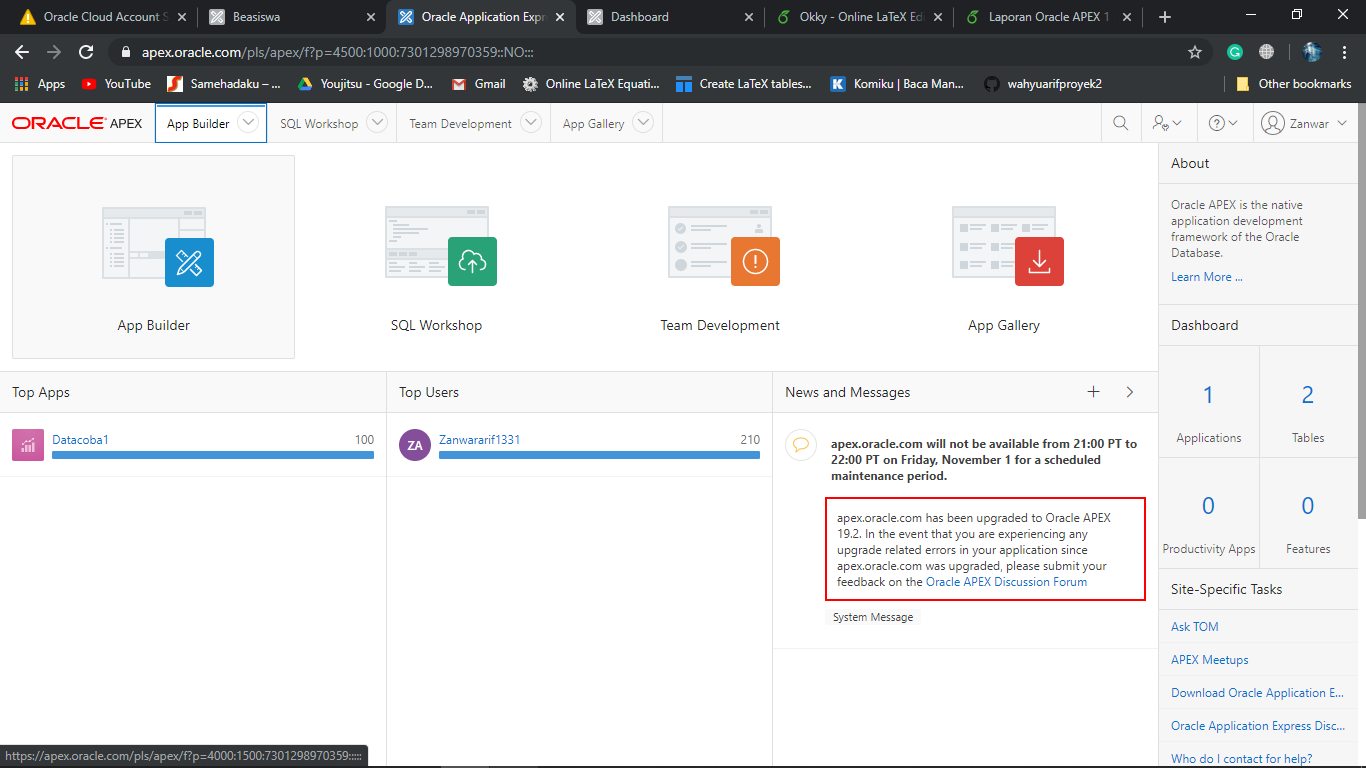
\includegraphics[scale=0.3]{figures/Screenshot(71).png}
        \caption{\textit{Home Oracle Application Express.}}
        \end{center}   
    \end{figure}
    
    \begin{figure}[!htbp]
    \item[2.] Pilih create pada menu aplikasi builder, kemudian kita akan menggunakan cara upload data yang sudah dari file excel.
        \begin{center}
        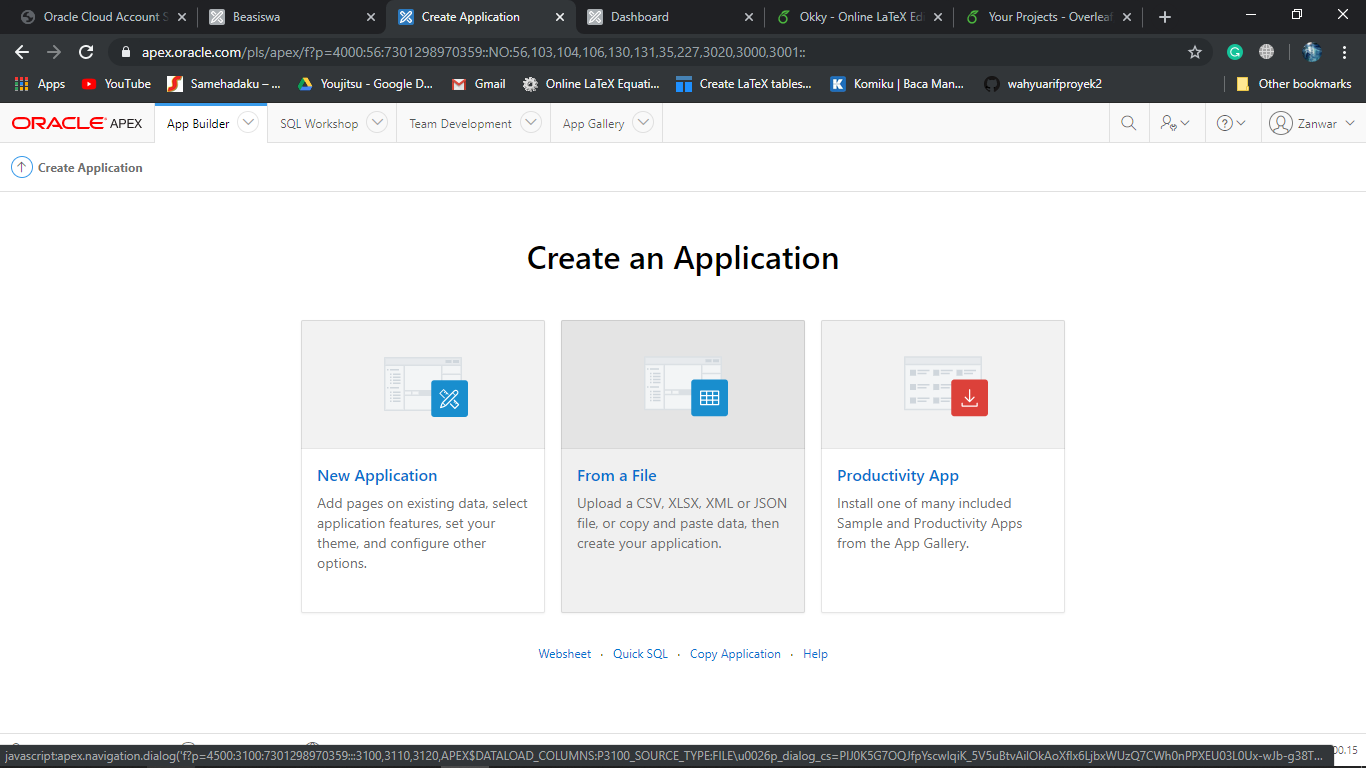
\includegraphics[scale=0.3]{figures/Screenshot(72).png}
        \caption{\textit{Create Application.}}
        \end{center}   
    \end{figure}

    \begin{figure}[!htbp]
    \item[3.] Kemudian pilih file yang akan diupload, tapi ingat filenya harus dengan ekstensi CSV,XLS,TXT,XML, dan JSON. Tapi disini kita mengupload file dengan ekstensi XLS.
        \begin{center}
        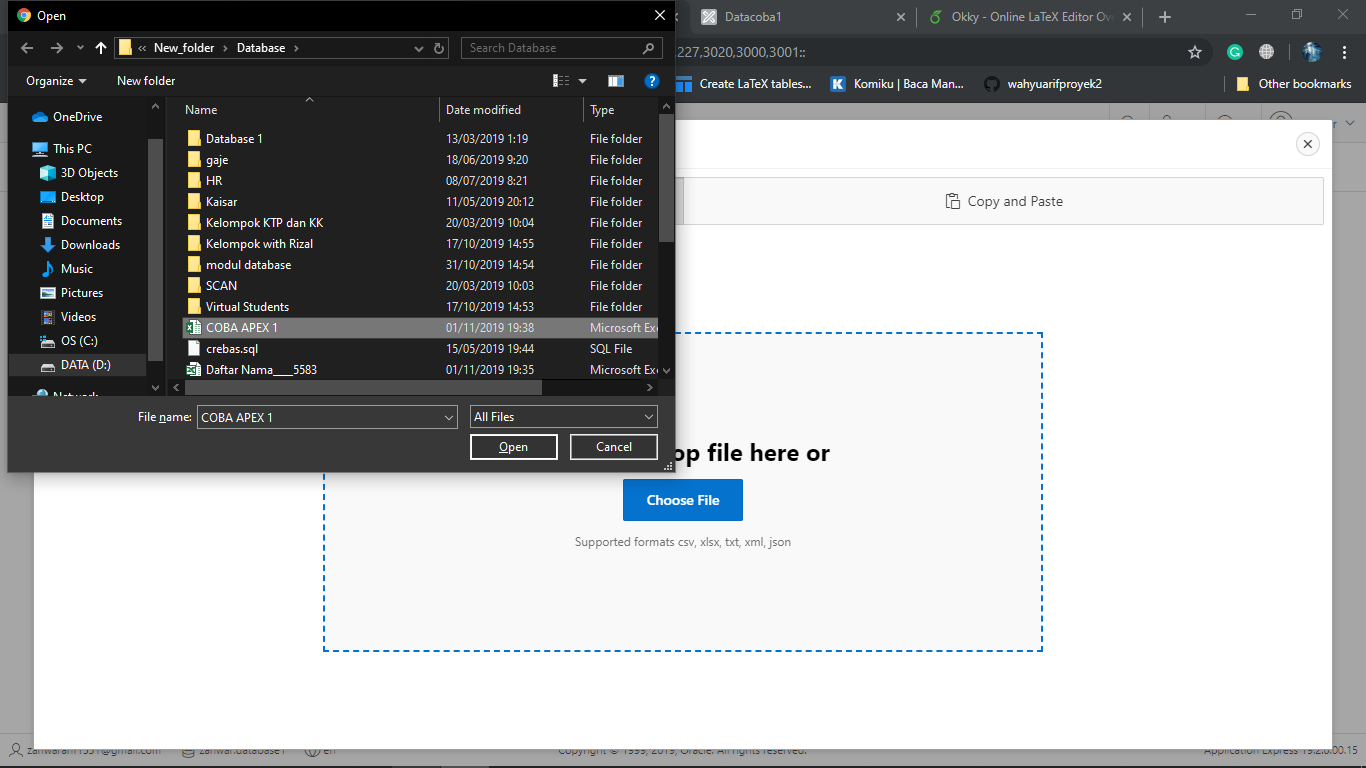
\includegraphics[scale=0.3]{figures/Screenshot(73).png}
        \caption{\textit{Choose File.}}
        \end{center}   
    \end{figure}
    
    \begin{figure}[!htbp]
    \item[4.] Setelah memilih file yang diupload, kita harus ememberikan nama tabel dari file yang kita upload.
    \begin{center}
    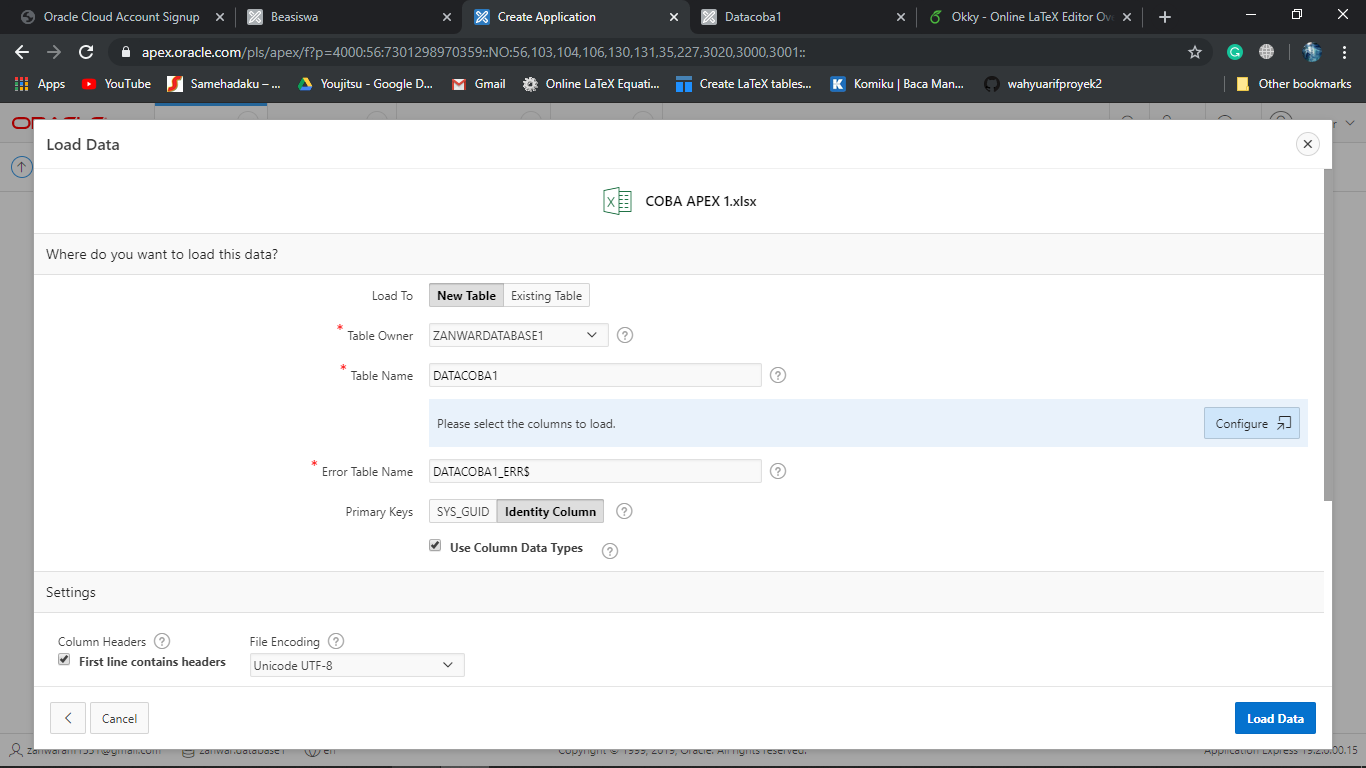
\includegraphics[scale=0.3]{figures/Screenshot(75).png}
    \caption{\textit{Load Data.}}
    \end{center}   
    \end{figure}
    
    \begin{figure}[!htbp]
    \item[5.] Selanjutnya kita juga bisa memastikan tabel yang kita upload seperti apa, apakah benar atau tidak ? Kita juga bisa mengatur attribut mana saja yang akan di tampilkan
    \begin{center}
    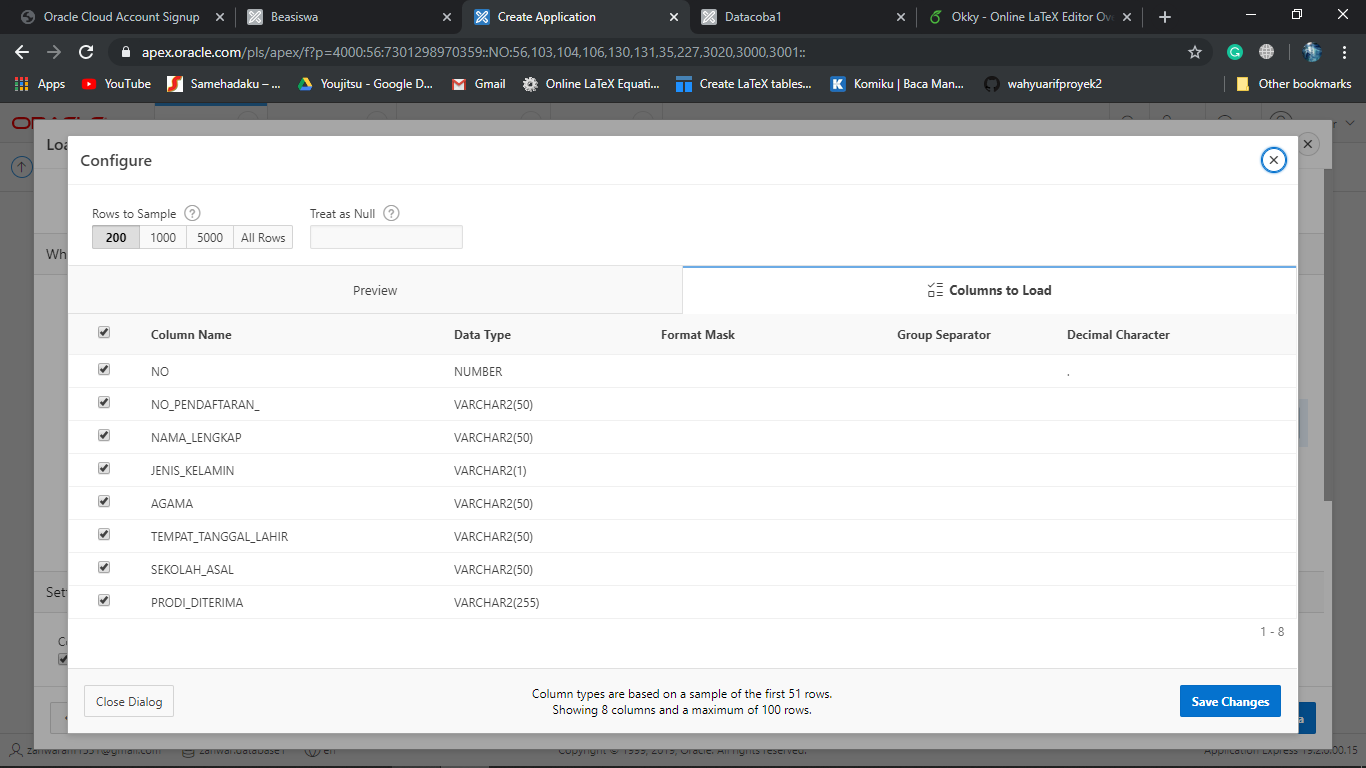
\includegraphics[scale=0.3]{figures/Screenshot(76).png}
    \caption{\textit{Configure Table 1.}}
    \end{center}   
    \end{figure}
    
    \begin{figure}[!htbp]
    \item[6.] Berikut bentuk tampilan tabel yang sudah kita upload.
    \begin{center}
    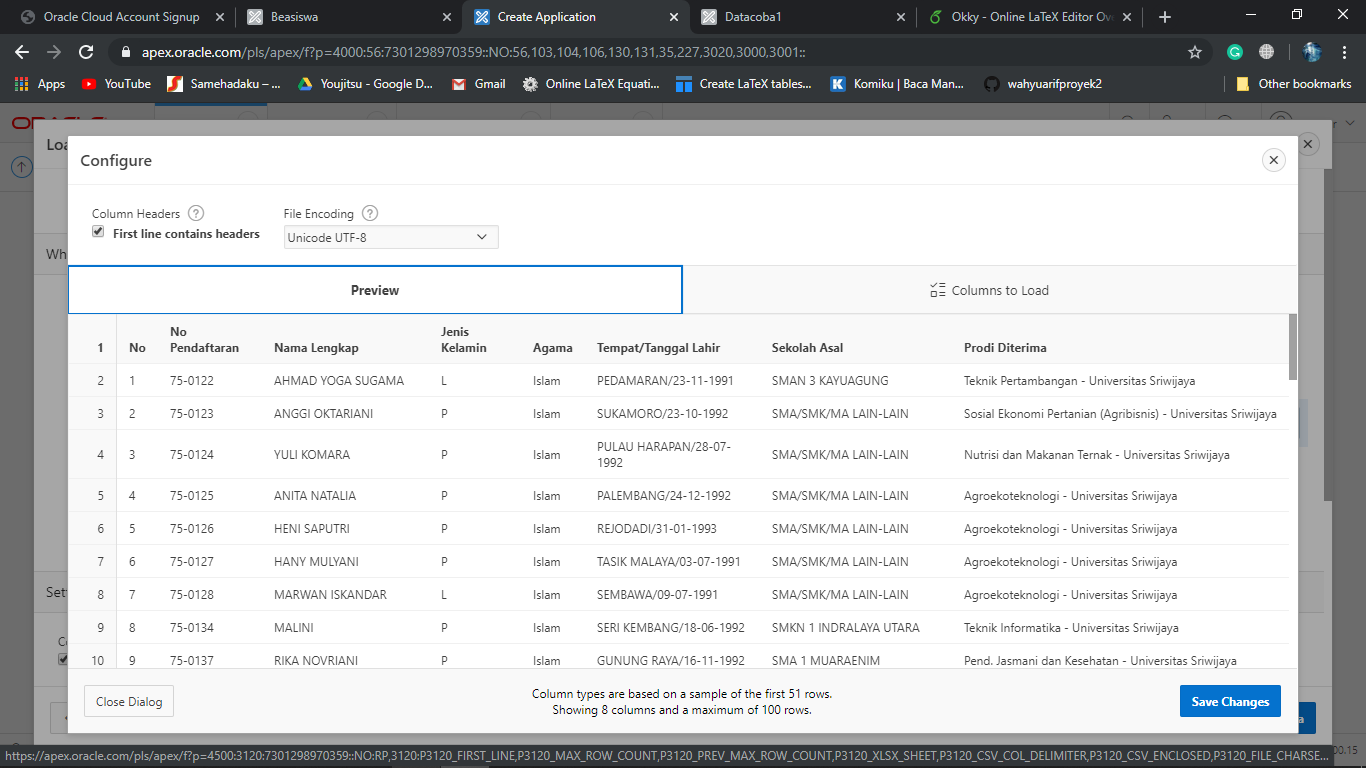
\includegraphics[scale=0.3]{figures/Screenshot(77).png}
    \caption{\textit{Configure Table 2.}}
    \end{center}   
    \end{figure}
    
    \begin{figure}[!htbp]
    \item[7.] Setelah memastikan tabel sudah benar kita bisa save, dan kemudian akan muncul proses pembuatan aplikasi, kita bisa melihat apa saja menu yang sudah disediakan oleh APEX, kemudian klik tombol CREATE APPLICATION di paling bawah.
    \begin{center}
    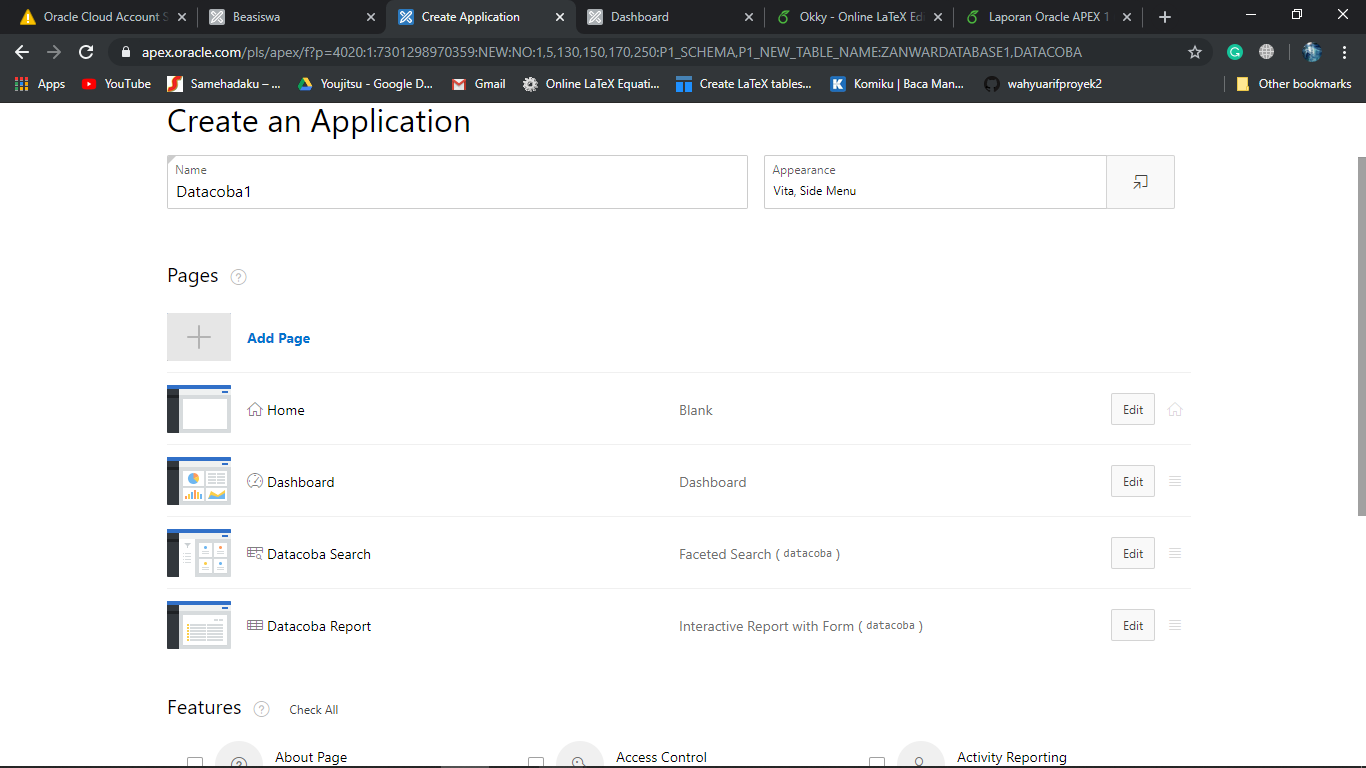
\includegraphics[scale=0.3]{figures/Screenshot(95).png}
    \caption{\textit{Create Application.}}
    \end{center}   
    \end{figure}
    
    \begin{figure}[!htbp]
    \item[8.] Tunggu APEX membuatkan aplikasi klean.
    \begin{center}
    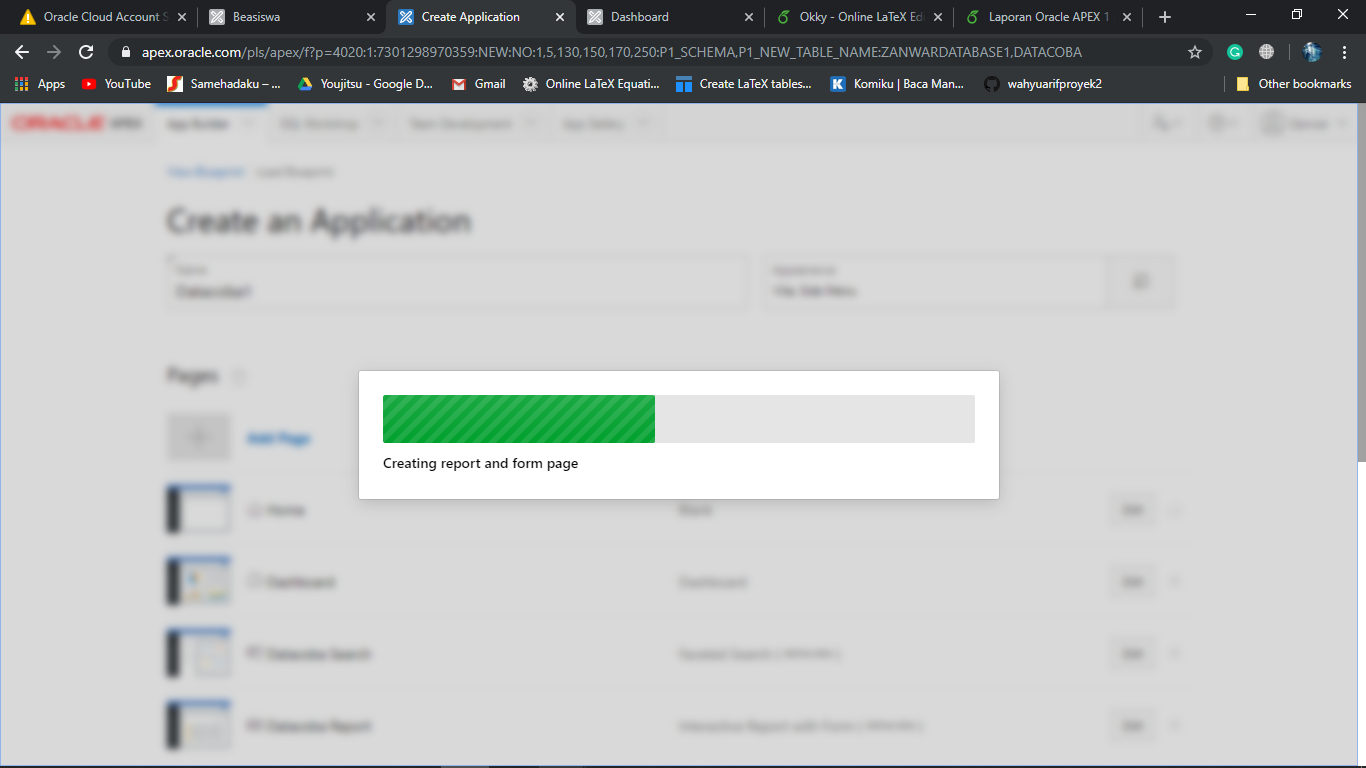
\includegraphics[scale=0.3]{figures/Screenshot(102).png}
    \caption{\textit{Loading Creat Application.}}
    \end{center}   
    \end{figure}
    
    \begin{figure}[!htbp]
    \item[9.] Setelah jadi kita bisa \textit{'Run'} aplikasi yang sudah kita buat.
    \begin{center}
    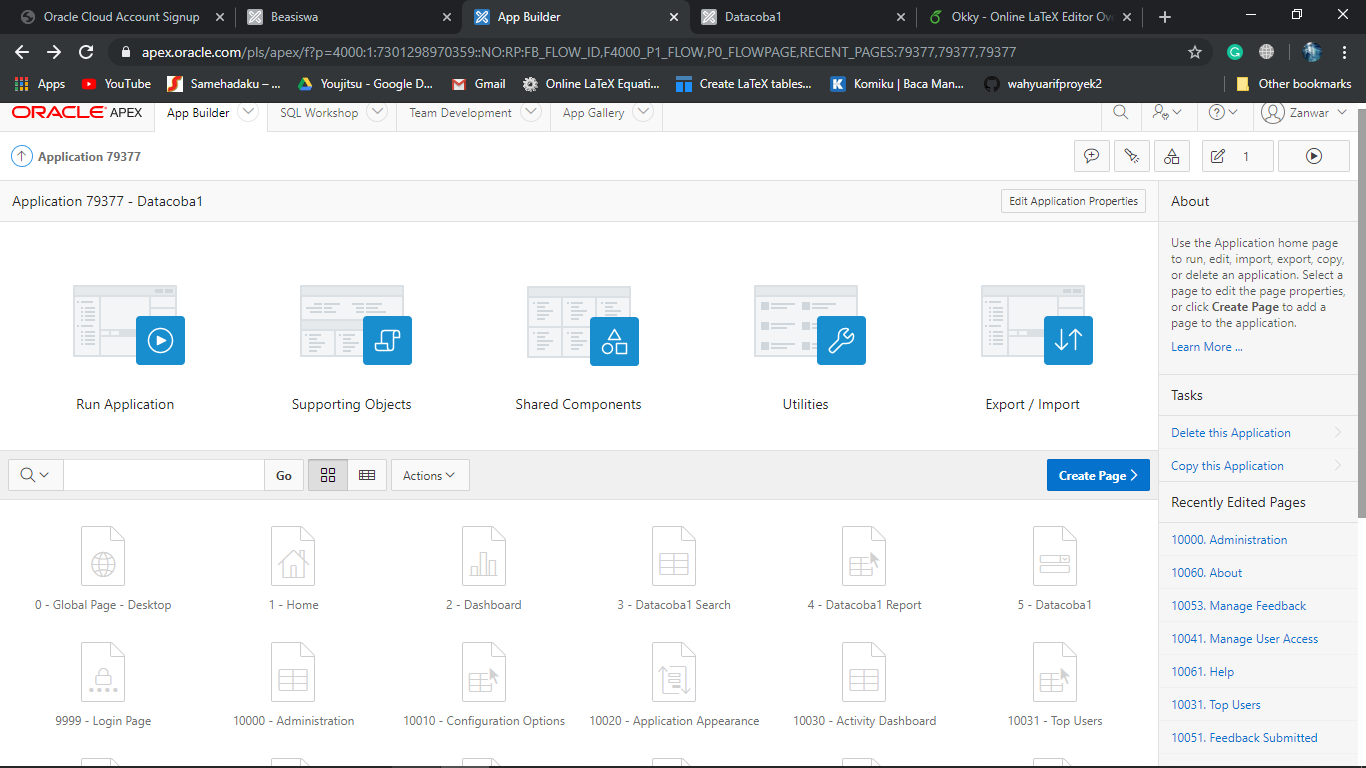
\includegraphics[scale=0.3]{figures/Screenshot(79).png}
    \caption{\textit{App Builder.}}
    \end{center}   
    \end{figure}
    
    \begin{figure}[!htbp]
    \item[10.] Berikut Tampilan Aplikasi yang berhasil kita buat.
    \par
    Sekian dari saya, bisa dilihat hasil aplikasi yang saya buat di link berikut. https://apex.oracle.com/pls/apex/f?p=34230:LOGIN\_DESKTOP:103665404926840:::::. 
    \par
    Login menggunakan akun email saya, zanwararif1331@gmail.com dengan password apajaboleh99
    \begin{center}
    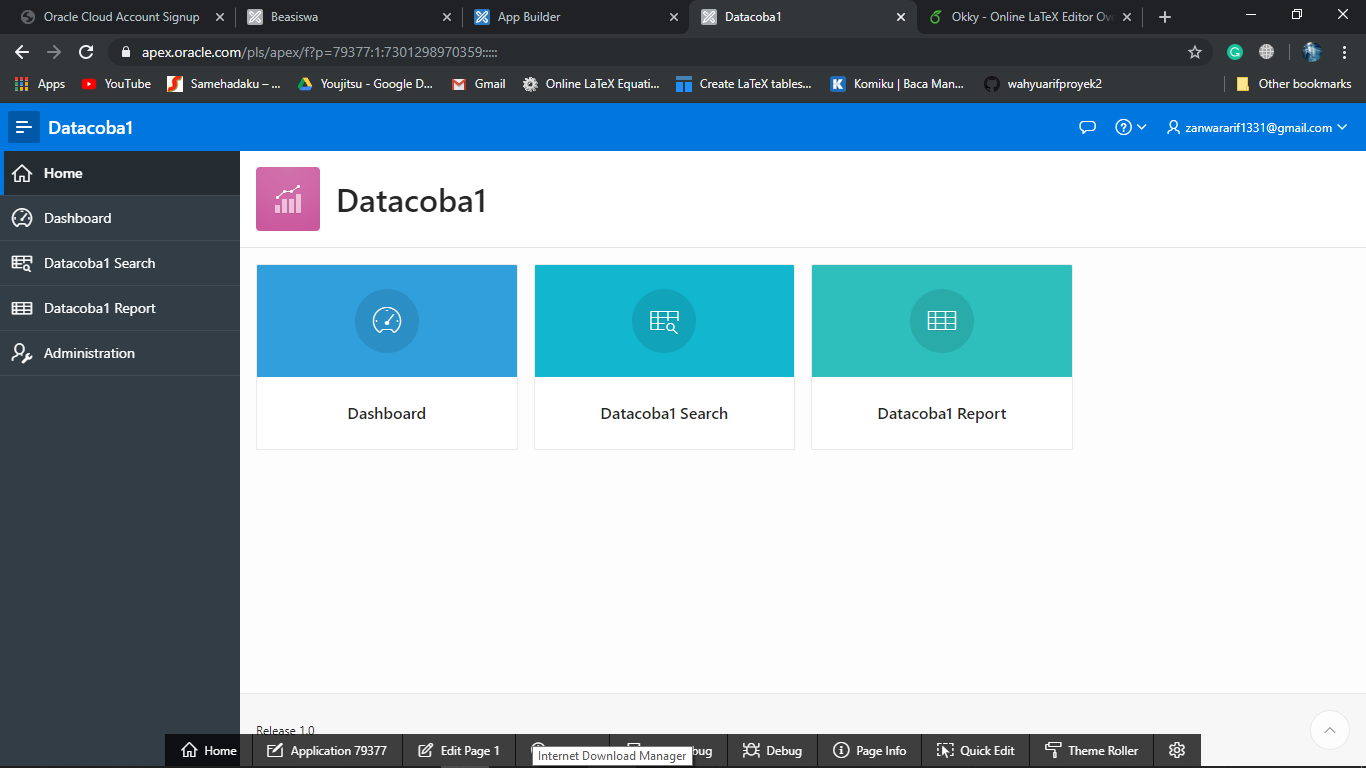
\includegraphics[scale=0.3]{figures/Screenshot(84).png}
    \caption{\textit{Get Start For Free.}}
    \end{center}   
    \end{figure}
    
\end{enumerate}

.